%!TEX TS-program = xelatex
%!TEX encoding = UTF-8 Unicode
\documentclass[russian,hyperref={unicode}]{beamer}
% Other packages (for math and grahics)
\usepackage{amsmath, amssymb, graphicx}
\graphicspath{{./images/}}
% Exclude backup slides from numbering
\usepackage{appendixnumberbeamer}
% Theme selection
\usetheme[sectionpage=none, numbering=fraction]{metropolis}
% Locale packages
\usepackage{polyglossia}
\setmainlanguage{russian}
\setotherlanguage{english}
\setkeys{russian}{babelshorthands=true}

\title{Способ определения координат и угловой ориентации бортовой пеленгаторной антенны по результатам радиопеленгования радиоориентиров}
\institute
{
  \inst{1}%
  Военно-воздушная академия имени профессора Н.Е.Жуковского и Ю.А.Гагарина\\
  \inst{2}%
	Воронежский Государственный Университет
}
\author
{
  Виноградов Д.А.\inst{1}, Минин Л.А.\inst{2}, Морозов Е.Ю.\inst{2}, Ушаков С.Н\inst{2}.
}
\date[RLNC 2019]{XXV Международная научно-техническая конференция <<Радиолокация, навигация, связь>>, 2019}

\begin{document}
  \frame{\titlepage}

  \section{Введение}
  \begin{frame}{Введение}
    Определение координат и угловой ориентации подвижных объектов производится с
    помощью GPS и ГЛОНАСС.

    Такие системы используют дальномерно-угломерный подход и работоспособны только
    при синхронном излучении радиосигналов радиоориентиров.

    Существуют угломерные системы, не накладывающие требований на синхронность излучения.

    Угломерные системы, способные однозначно и одновременно определять координаты и
    угловую ориентацию подвижного объекта только с помощью азимутально-угломестного
    радиопеленгования радиоориетиров, не исследованы.
  \end{frame}

  \section{Постановка задачи}
  \begin{frame}{Постановка задачи}
      Пусть $N$ радиоориентиров размещены в точках пространства с известными координатами.

      Подвижный объект оснащен бортовой пеленгаторной антенной, способной для каждого
      РО определить азимут и угол места в связанной системе координат.

      Необходимо определить пространственную ориентацию подвижного объекта,
      используя минимальное число РО.
  \end{frame}

  \begin{frame}{Постановка задачи}
    Всего необходимо определить шесть параметров "--- три координаты и три угла Эйлера,
    определяющих угловую ориентацию подвижного объекта.

    БПА подвижного объекта измеряет два параметра для каждого из радиоориентиров "---
    азимут и угол места.

    Таким образом, минимальное число РО равно трем.
  \end{frame}

  \begin{frame}{Постановка задачи}
    \begin{figure}
      \begin{center}
        \includegraphics[width=.8\textheight]{tetrahedron}

        \caption{Схема размещения в пространстве трех радиоориентиров $M_1$, $M_2$ и $M_3$ и подвижного объекта $M_0$}
      \end{center}
    \end{figure}
  \end{frame}

  \begin{frame}{Схема решения}
    Можно выделить три этапа решения задачи:
    \begin{enumerate}
        \item Нахождение совокупности расстояний от подвижного объекта до радиоориентиров;
        \item Определение координат подвижного объекта;
        \item Нахождение матрицы вращения и связанных с нею углов Эйлера, определяющих угловую ориентацию подвижного объекта.
    \end{enumerate}
    Задачи второго и третьего этапов являются стандартными для радионавигации подвижных объектов.
  \end{frame}

  \begin{frame}{Схема решения}
    Система уравнений для нахождения расстояний (этап 1):
    \begin{equation} \label{eq:system}
      \begin{cases}
        \ell_1^2 + \ell_2^2 - 2 \ell_1 \ell_2 \cos\alpha_{12} = d_{12}^2 \\
        \ell_1^2 + \ell_3^2 - 2 \ell_1 \ell_3 \cos\alpha_{13} = d_{13}^2 \\
        \ell_2^2 + \ell_3^2 - 2 \ell_2 \ell_3 \cos\alpha_{23} = d_{23}^2
      \end{cases}
    \end{equation}
    Нелинейная, однородная система второго порядка.
  \end{frame}

  \begin{frame}{Схема решения}
    Представим, что объект поднимается вверх относительно плоскости радиоориентиров.

    До определенной критической высоты, система~(\ref{eq:system}) имеет единственное решение.

    Начиная с первой критической высоты, из одной из вершин выходит первое <<паразитное>>
    решение.

    Всего система~(\ref{eq:system}) может иметь от одного до четырех решений.
    % TODO: рисунок из математики?
  \end{frame}

  \section{Особенности решения}
  \begin{frame}{Особенности решения. Первый этап}
    Как показали вычислительные эксперименты, произведенные в пакете Mathematica,
    увеличение числа РО не приводит к улучшению разрешимости.

    В этом случае система становится переопределенной, а с учетом погрешностей измерений "---
    несовместной.

    Функционал МНК минимизации невязки в квадрате приводит к системе уравнений третьего порядка
    и усложнению вычислений.
  \end{frame}

  \begin{frame}{Особенности решения. Первый этап}
    Систему~(\ref{eq:system}) можно решать методом Ньютона. Это обусловлено следующим:
    \begin{itemize}
      \item Имеется хорошее начальное приближение
      \item Быстрая сходимость к решению (5-10 итераций)
      \item В реализации присутствуют только элементарные арифметические действия "--- обратная
            матрица выписывается явно
    \end{itemize}
  \end{frame}

  \begin{frame}{Особенности решения. Второй этап}
    После нахождения расстояний, координаты подвижного объекта можно найти из следующей
    системы уравнений:

    \begin{equation}\label{eq:system_coordinates}
      \begin{cases}
        \left(x_1 - x\right)^2 + \left(y_1 - y\right)^2 + \left(z_1 - z\right)^2 = \ell_1^2 \\
        \left(x_2 - x\right)^2 + \left(y_2 - y\right)^2 + \left(z_2 - z\right)^2 = \ell_2^2 \\
        \left(x_3 - x\right)^2 + \left(y_3 - y\right)^2 + \left(z_3 - z\right)^2 = \ell_3^2
      \end{cases}
    \end{equation}

    Интересно, что удобнее решать систему~(\ref{eq:system_coordinates}) в системе координат,
    связанной с плоскостью радиоориентиров "--- в таком случае, нахождение координат
    существенно упрощается.
  \end{frame}

  \section{Заключение}
  \begin{frame}{Оценка погрешностей}
    Осложняется следующими факторами:
    \begin{itemize}
      \item Система уравнений~(\ref{eq:system}) может иметь до четырех решений
      \item Система уравнений~(\ref{eq:system}) решается итерационным методом
      \item Точность решения зависит от конфигурации системы
      \item Подвижный объект может находиться около точек бифуркации
    \end{itemize}

    Параллельно в работе [1] был проведен анализ погрешностей, используя метод
    максимального правдоподобия, подтверждающий аналитические выводы данной работы.
  \end{frame}

  \begin{frame}{Дальнейшие планы}
    Параллельно с этой системой, ведутся исследования других конфигураций, к примеру,
    с несколькими подвижными объектами.

    Пока эта модель "--- единственная, в которой подвижный объект способен работать в
    пассивном режиме, не обмениваясь информацией с радиоориентирами.
  \end{frame}

  \frame{\titlepage}

  \appendix
  \begin{frame}{Визуализация решений, полученных на первом этапе}
    \begin{columns}[c]
      \begin{column}{.5\textwidth}
        \begin{itemize}
          \item В основании "--- равносторонний треугольник
          \item Аппарат изначально находился в центре
          \item Фиолетовым цветом выделены зоны с одним решением
          \item Оранжевым "--- зоны с несколькими решениями
        \end{itemize}
      \end{column}
      \begin{column}{.5\textwidth}
        \begin{center}
          \includegraphics[width=\columnwidth]{tetrahedron-regular}
        \end{center}
      \end{column}
    \end{columns}
  \end{frame}

  \begin{frame}{Визуализация решений, полученных на первом этапе}
    \begin{columns}[c]
      \begin{column}{.5\textwidth}
        \begin{itemize}
          \item В основании также равносторонний треугольник
          \item Аппарат изначально находился рядом с одной из вершин
        \end{itemize}
      \end{column}
      \begin{column}{.5\textwidth}
        \begin{center}
          \includegraphics[width=\columnwidth]{tetrahedron-bifurcation}
        \end{center}
      \end{column}
    \end{columns}
  \end{frame}

  \begin{frame}{Визуализация решений, полученных на первом этапе}
    \begin{columns}[c]
      \begin{column}{.5\textwidth}
        \begin{itemize}
          \item В основании также равносторонний треугольник
          \item Аппарат изначально находился за пределами треугольника
          \item При дальнейшем подъеме аппарата паразитные имеют
                сложную структуру
        \end{itemize}
      \end{column}
      \begin{column}{.5\textwidth}
        \begin{center}
          \includegraphics[height=.9\textheight]{tetrahedron-away}
        \end{center}
      \end{column}
    \end{columns}
  \end{frame}

  \begin{frame}{Геометрическая интерпретация решений}
    Рассмотрим треугольник, образованный двумя РО ($M_i$, $M_j$) и подвижным объектом $M_0$.

    Так как известен угол $\angle M_i M_0 M_j$, точка $M_0$ может лежать на окружности с хордой $M_i$ $M_j$.

    Геометрическое место точек, в которых может находится $M_0$ при заданных $\ell_{i}$, $\ell_{j}$ и
    $\angle M_i M_0 M_j$ образуется вращением этой окружности вокруг хорды $M_i$ и $M_j$, образуя \textit{закрытый тор}.

    Пересечение трех закрытых торов, полученных для каждой из сторон, является истинным положением
    воздушного объекта.
  \end{frame}

  \begin{frame}{Геометрическая интерпретация решений}
    \begin{center}
      \begin{figure}
        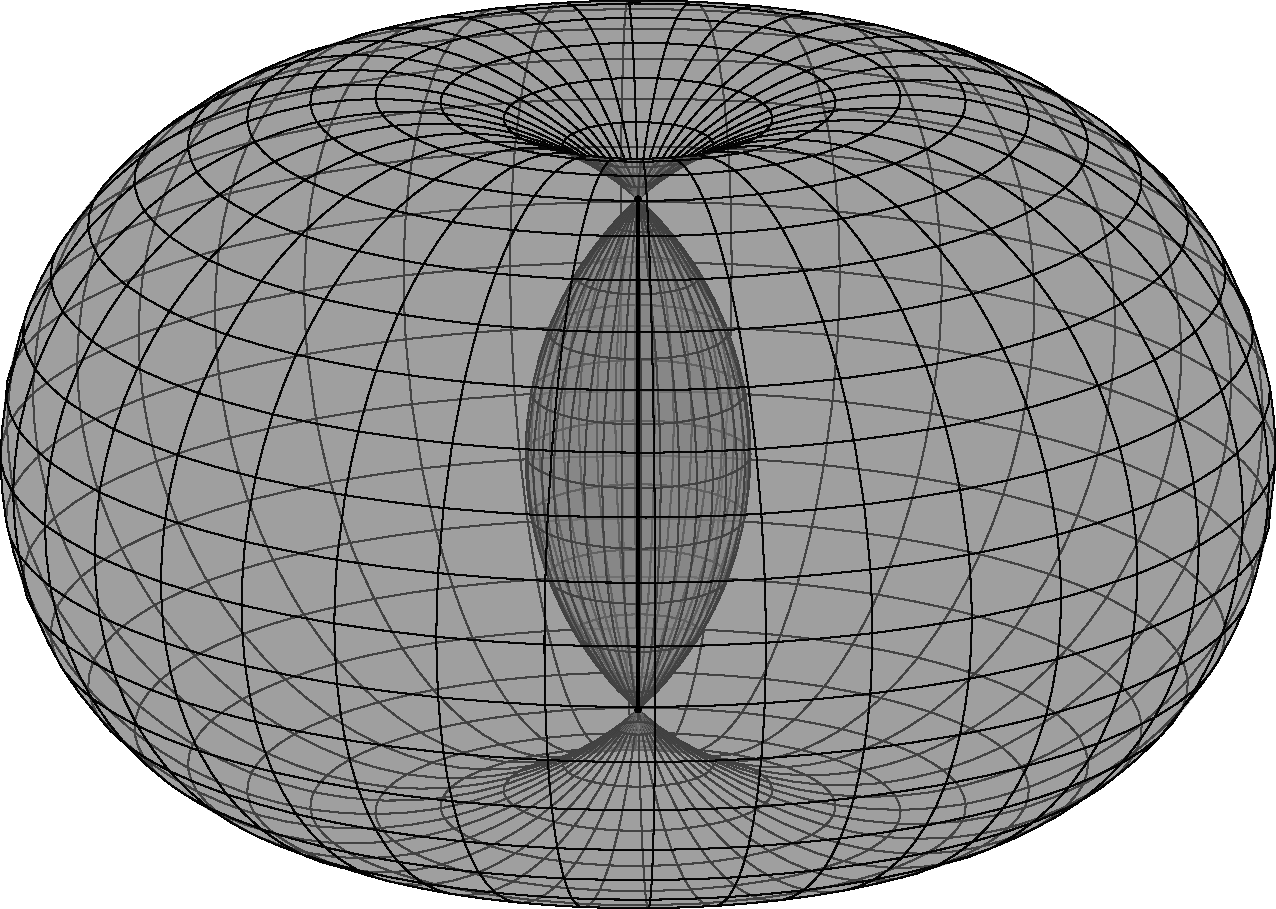
\includegraphics[height=.7\textheight]{torus}
        \caption{Закрытый тор, иллюстрирующий области возможного нахождения подвижного объекта $M_0$
        относительно ребра $M_1M_2$.}
      \end{figure}
    \end{center}
  \end{frame}
\end{document}
